% Бүлэг 2

\chapter{Системийн шинжилгээ ба загварчлал} % Бүлгийн нэр
\label{Chapter2} % Энэ бүлэг рүү ишлэл хийх бол \ref{Chapter1} командыг ашигла 


\section{ Хэрэглэгчийн шаардлага }
\subsection{Системийг ашиглах хэрэглэгчид}
    \begin{itemize}
    \item Админ
    \item Хэрэглэгч
    \item Зочин
\end{itemize}

\subsection{Системийн хэрэглэгчид дэлгэрэнгүй}
\text{Манай систем нь 3 түвшний хэрэглэгчтэй}
\begin{itemize}
    \item \textbf{Админ}
    \par\noindent Энэ хэрэглэгч нь системийг удирдах, хэрэглэгчдийг удирдах, бараа удирдах зэрэг удирдлагын чанартай хамгийн дээд түвшний эрхтэй хэрэглэгч юм.
    \item \textbf{Хэрэглэгч}
    \par\noindent Энэхүү хэрэглэгч нь өөрийн худалдаалахыг хүссэн барааг дуудлага худалдаанд байршуулах, бусад хэрэглэгчийн барааг дуудлага худалдаанаас худалдан авах боломжтой системд бүртгэлтэй хэрэглэгч юм.
    \item \textbf{Зочин}
    \par\noindent Энэхүү хэрэглэгч нь хэдийд ч, хаанаас ч дуудлага худалдаанд байгаа барааг харах танилцах болон системд бүртгүүлэх боломжтой системд бүртгэлгүй хэрэглэгч юм. 
\end{itemize}
\newpage
    \section{Системийн функциональ шаардлага}
    \subsection{Админы функциональ шаардлага}
    1. Бараа зохицуулалт
    \begin{itemize}
    \item Бараа устгах
    \item Бараа нэмэх 
    \item Барааны мэдээлэл засах
    \item Бараа худалдах
\end{itemize}
      2. Хэрэглэгч удирдах
    \begin{itemize}
    \item хайлт хийх 
    \item хэрэглэгчийн бараа үзэх
    \end{itemize}
    3. Худалдаануудын мэдээллийг харах
    \par\noindent 4. Хэрэглэгчдийн дансыг цэнэглэх
    \par\noindent 5. Системд нэвтрэх
    \par\noindent 6. Ангилал удирдах
    \begin{itemize}
    \item Ангилал устгах
    \item Ангилал нэмэх 
\end{itemize}
   \par\noindent 7. Ирсэн хүсэлтүүдийг зохицуулах
   \begin{itemize}
    \item Хүсэлтийг зөвшөөрөх
    \item Хүсэлтийг татгалзах 
\end{itemize}
    \subsection{Хэрэглэгчийн функциональ шаардлага}
    1. Бараа зохицуулалт
    \begin{itemize}
    \item Бараа устгах
    \item Бараа нэмэх 
    \item Барааны мэдээлэл засах
    \item Бараа худалдах
\end{itemize}
     \par\noindent 2. Профайл удирдах - Жишээ нь: Нууц үг солих 
     \par\noindent 3. Системд нэвтрэх
     \par\noindent 4. бараа хайх
     \begin{itemize}
    \item Энгийн хайлт хийх
    \item Шүүлтүүр тавин хайлт хийх
\end{itemize}
     \par\noindent 5. Бараа үзэх
     \par\noindent 6. Данс цэнэглэх
     \par\noindent 7. Худалдан авалтын түүх харах
     \par\noindent 8. Үнэ санал болгох
     \par\noindent 9.  Худалдан авалт хийх 
    \subsection{Зочны функциональ шаардлага}
    1. Идэвхтэй дуудлага худалдаануудыг үзэх
    \par\noindent 2. бараа хайх
     \begin{itemize}
    \item Энгийн хайлт хийх
    \item Шүүлтүүр тавин хайлт хийх
\end{itemize}
\par\noindent 3.Бүртгэл үүсгэх
\par\noindent 4.Нэвтрэх

\newpage
 \section{Системийн функциональ бус шаардлага}
    \subsection{Гүйцэтгэлийн шаардлага}
    1. Хялбар хурдан хайлт хийх
    \begin{itemize}
    \item Хуудас шилжих хугацаа 5 секундээс хэтрэхгүй байх
\end{itemize}
    \par\noindent 2. Хэрэглэхэд ойлгомжтой хялбар байх
    \begin{itemize}
    \item Хэрэглэгч хараад ойлгомжтой байхаар хөгжүүлнэ
    \item Дуудлага худалдаанд үнэ өгөх болон хугацааг харуулах хэсгийг real-time data ашиглана гүйцэтгэх
\end{itemize}
    \par\noindent 3. Системийн хариу өгөхөд бага хугацаа зарцуулдаг байх
    \begin{itemize}
    \item 5 секундээс ихгүй байх
\end{itemize}
    \par\noindent 4. Сервер нь 24/7 цагийн ажиллагаатай байх
    \begin{itemize}
    \item 24 цагаар худалдан авагч болон худалдаалагчдад үйлчилгээг үзүүлэх
\end{itemize}
    \subsection{ Программ хангамжийн шинж чанарууд}
  
    \par\noindent 1. Хүртээмжтэй байдал
    \begin{itemize}
    \item Сервер унасан үед нөөц сервер лүү шилжих
\end{itemize}
    \par\noindent 2. Аюулгүй байдал
    \begin{itemize}
    \item Нууц үгээ шифрлэлт хийж хадгалах
 
\end{itemize}
\newpage
\section{Системийн архитектур}

Энэхүү систем нь 3 давхаргат (3-tier) full-stack архитектуртай бөгөөд дараах үндсэн бүрэлдэхүүн хэсгүүдээс бүрдэнэ:
\begin{figure}[htbp]
    \centering
    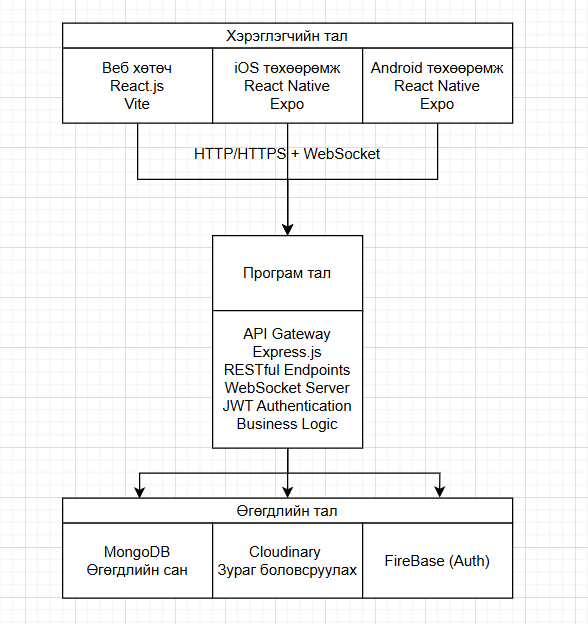
\includegraphics[width=1\linewidth]{Chart/3 tier.png}
    \caption{Enter Caption}
    \label{fig:placeholder}
\end{figure}

\subsection{Client тийн давхарга (Presentation Layer)}

\begin{itemize}
    \item \textbf{Веб клиент}: React.js + Vite ашиглан хөгжүүлсэн Single Page Application (SPA). Responsive дизайнтай, бүх төхөөрөмж дээр тохируулга хийх боломжтой.
    \item \textbf{Мобайл клиент}: React Native + Expo ашиглан хөгжүүлсэн cross-platform мобайл аппликейшн. iOS болон Android төхөөрөмж дээр native performance-тай ажиллана.
    \item \textbf{Харилцааны протокол}: RESTful API (HTTP/HTTPS), WebSocket (Socket.io) - бодит цагийн мэдээлэл солилцох
\end{itemize}

\subsection{Бизнес логикийн давхарга (Application Layer)}
\begin{itemize}
    \item \textbf{Backend API}: Node.js + Express.js framework дээр бүтээгдсэн RESTful API сервер
    \item \textbf{Үндсэн функцүүд}:
    \begin{itemize}
        \item Хэрэглэгчийн баталгаажуулалт (JWT, Google OAuth, Firebase Phone Auth)
        \item Бараа удирдах (CRUD үйлдлүүд, зураг хадгалалт)
        \item Дуудлага худалдааны логик (санал авах, дуудлага худалдааны статус шалгах)
        \item Бодит цагийн мэдээлэл дамжуулалт (Socket.io)
        \item Гүйлгээ болон төлбөрийн системийн интеграци
    \end{itemize}
    \item \textbf{Middleware}: Authentication, Authorization, Error handling, Rate limiting
\end{itemize}

\subsection{Өгөгдлийн давхарга (Data Layer)}
\begin{itemize}
    \item \textbf{Өгөгдлийн сан}: MongoDB (NoSQL) - уян хатан схем, өргөтгөх боломжтой
    \item \textbf{Өгөгдлийн модел}: User, Product, Bidding, Transaction, Category, Notification гэх мэт
    \item \textbf{Хадгалах систем}:
    \begin{itemize}
        \item Өгөгдлийн сан: MongoDB Atlas (cloud database)
        \item Зураг хадгалалт: Cloudinary эсвэл локал файлын систем
    \end{itemize}
\end{itemize}

\subsection{Системийн харилцааны бүтэц}
Бүх клиент (веб болон мобайл) нь нэгэн backend API руу хандаж мэдээлэл солилцдог. Энэ нь:
\begin{itemize}
    \item Кодыг давхардуулахаас сэргийлнэ (DRY principle)
    \item Бизнес логикийг төвлөрсөн удирдлага хийнэ
    \item Аюулгүй байдлыг төвлөрсөн хэрэгжүүлнэ
    \item Өргөтгөх, засвар хийхэд хялбар болгоно
\end{itemize}

Бодит цагийн функцүүд (дуудлага худалдааны мэдээлэл, мэдэгдэл) нь Socket.io ашиглан WebSocket холболтоор дамждаг. Бусад үйлдлүүд нь REST API ашиглана.

\clearpage

\section{ERD (Entity Relation Diagram)}
\begin{figure}[htbp]
    \centering
    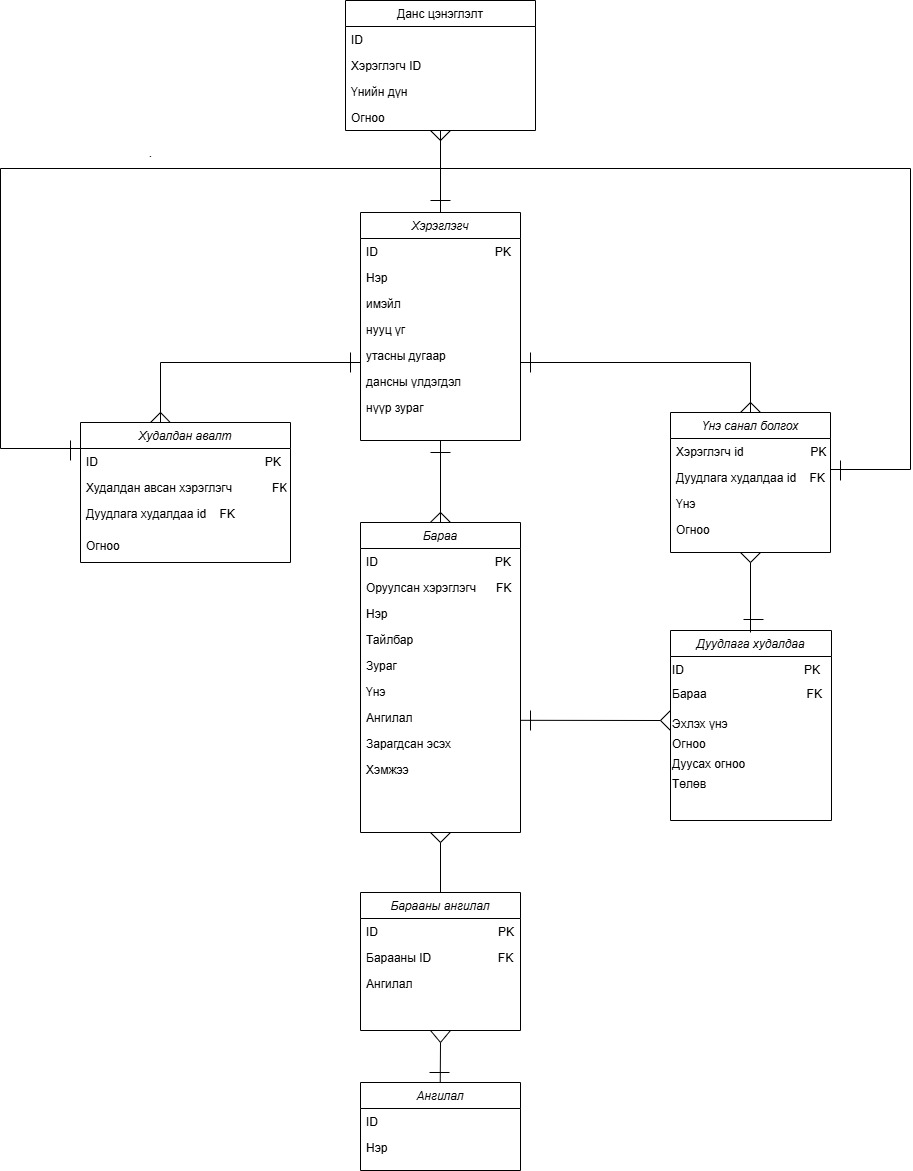
\includegraphics[width=0.9\textwidth]{Diagrams/erd}
    \caption{Өгөгдлийн хамаарлын диаграм (ERD)}
    \label{fig:erd}
\end{figure}
\clearpage

\section{Класс диаграм}
\begin{figure}[htbp]
    \centering
    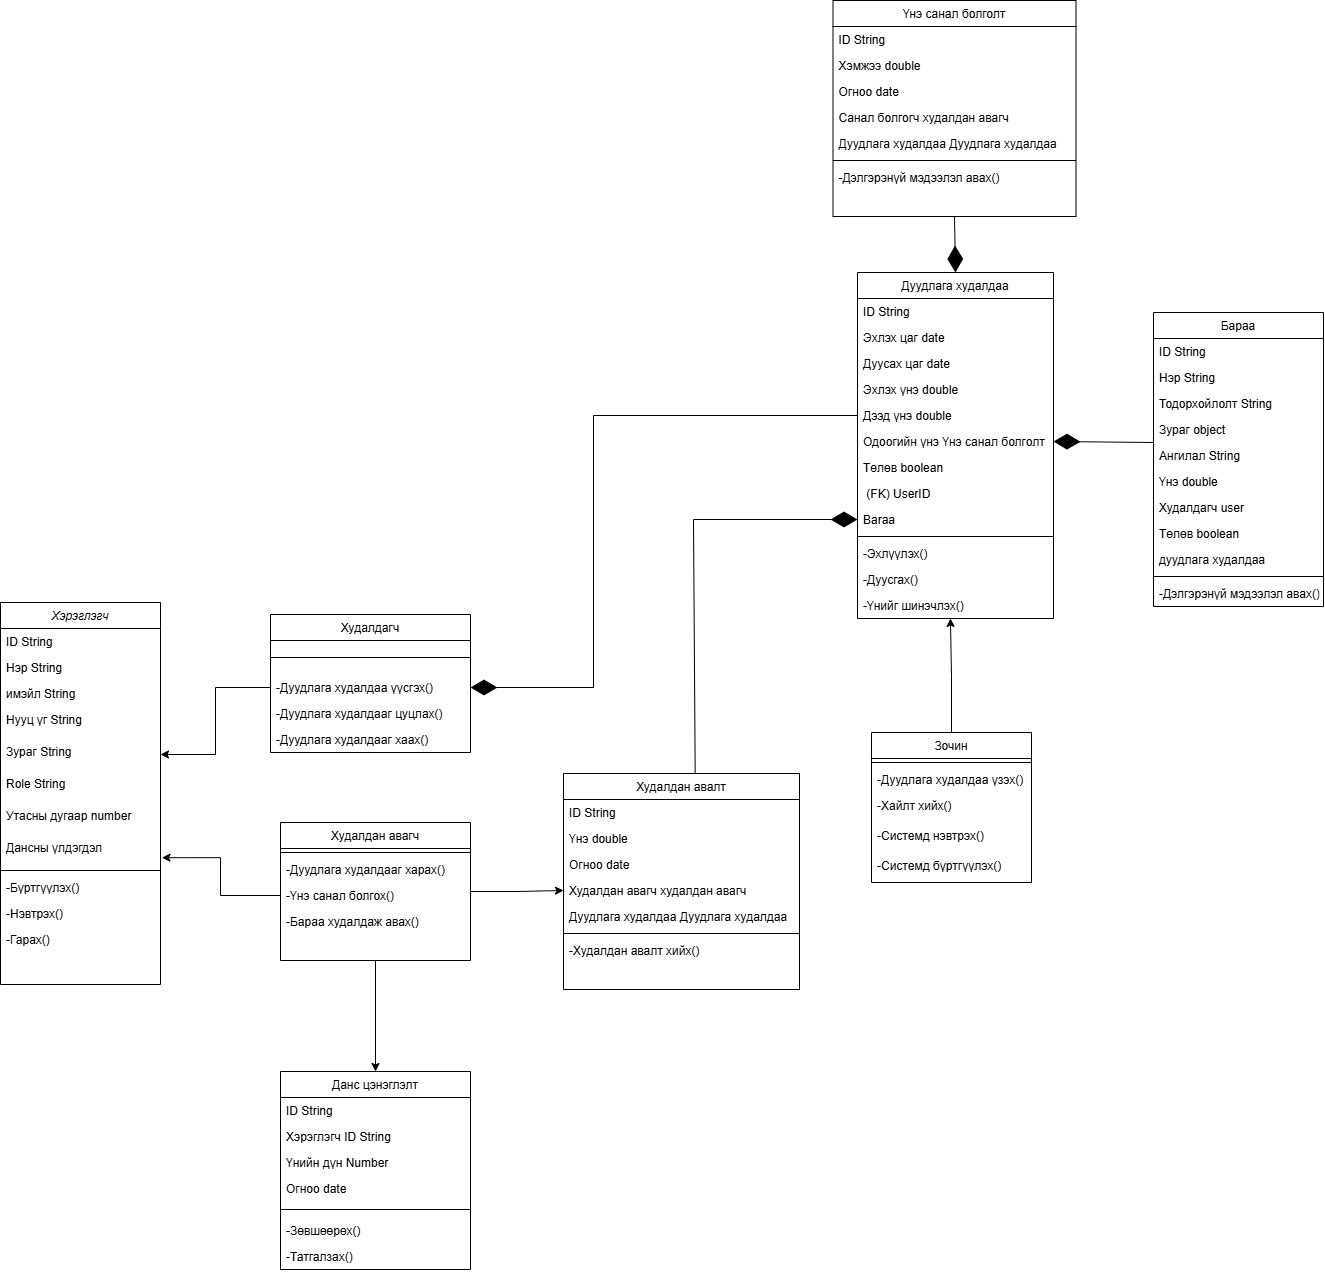
\includegraphics[width=0.9\textwidth,angle=0]{Diagrams/ClassDiagramm.jpg}
    \caption{Зохиомжийн шатны класс диаграм}
    \label{fig:class}
\end{figure}
\clearpage

\section{Дарааллын диаграм}
\begin{figure}[htbp]
    \centering
    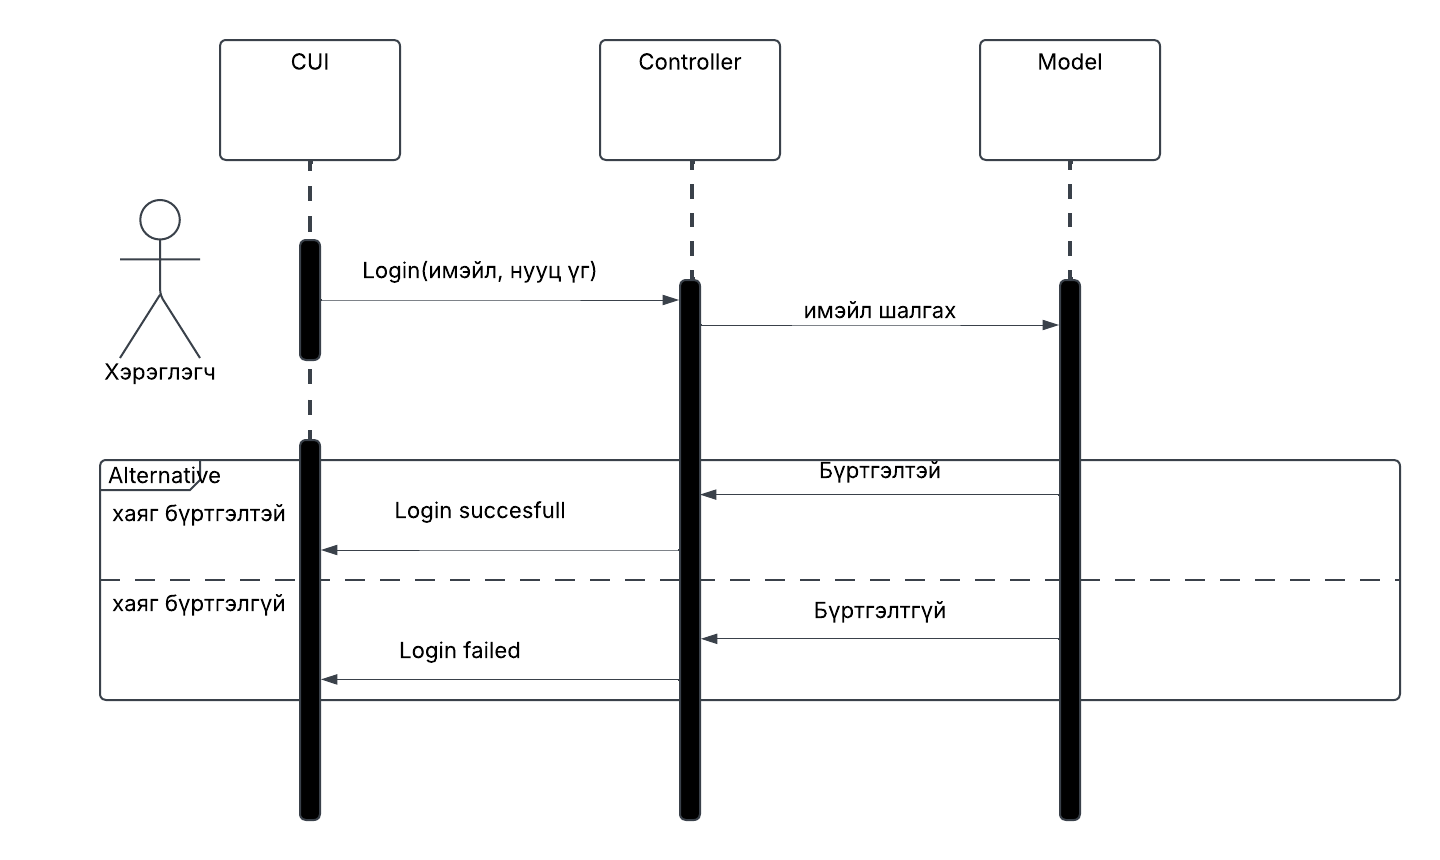
\includegraphics[width=0.9\textwidth]{Diagrams/login}
    \caption{Нэвтрэх дарааллын диаграм}
    \label{fig:login}
\end{figure}

\begin{figure}[htbp]
    \centering
    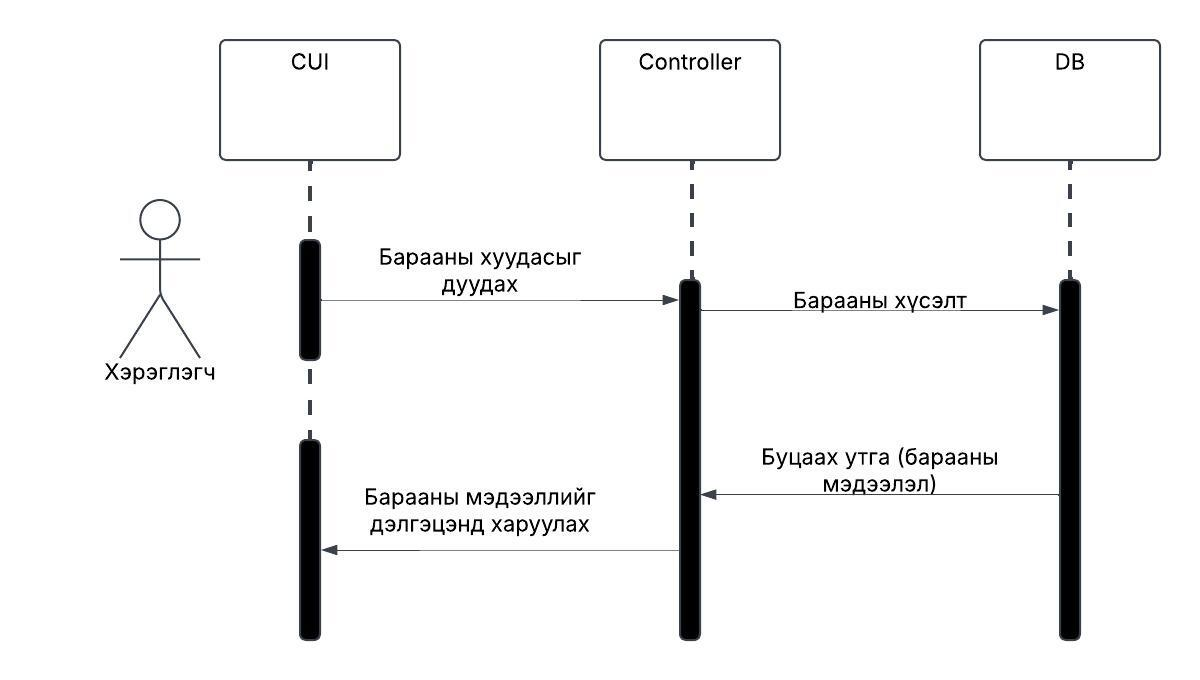
\includegraphics[width=0.9\textwidth]{Diagrams/baraauzeh}
    \caption{Дуудлага худалдаа үзэх дарааллын диаграм}
    \label{fig:comment}
\end{figure}
\clearpage

\begin{figure}[htbp]
    \centering
    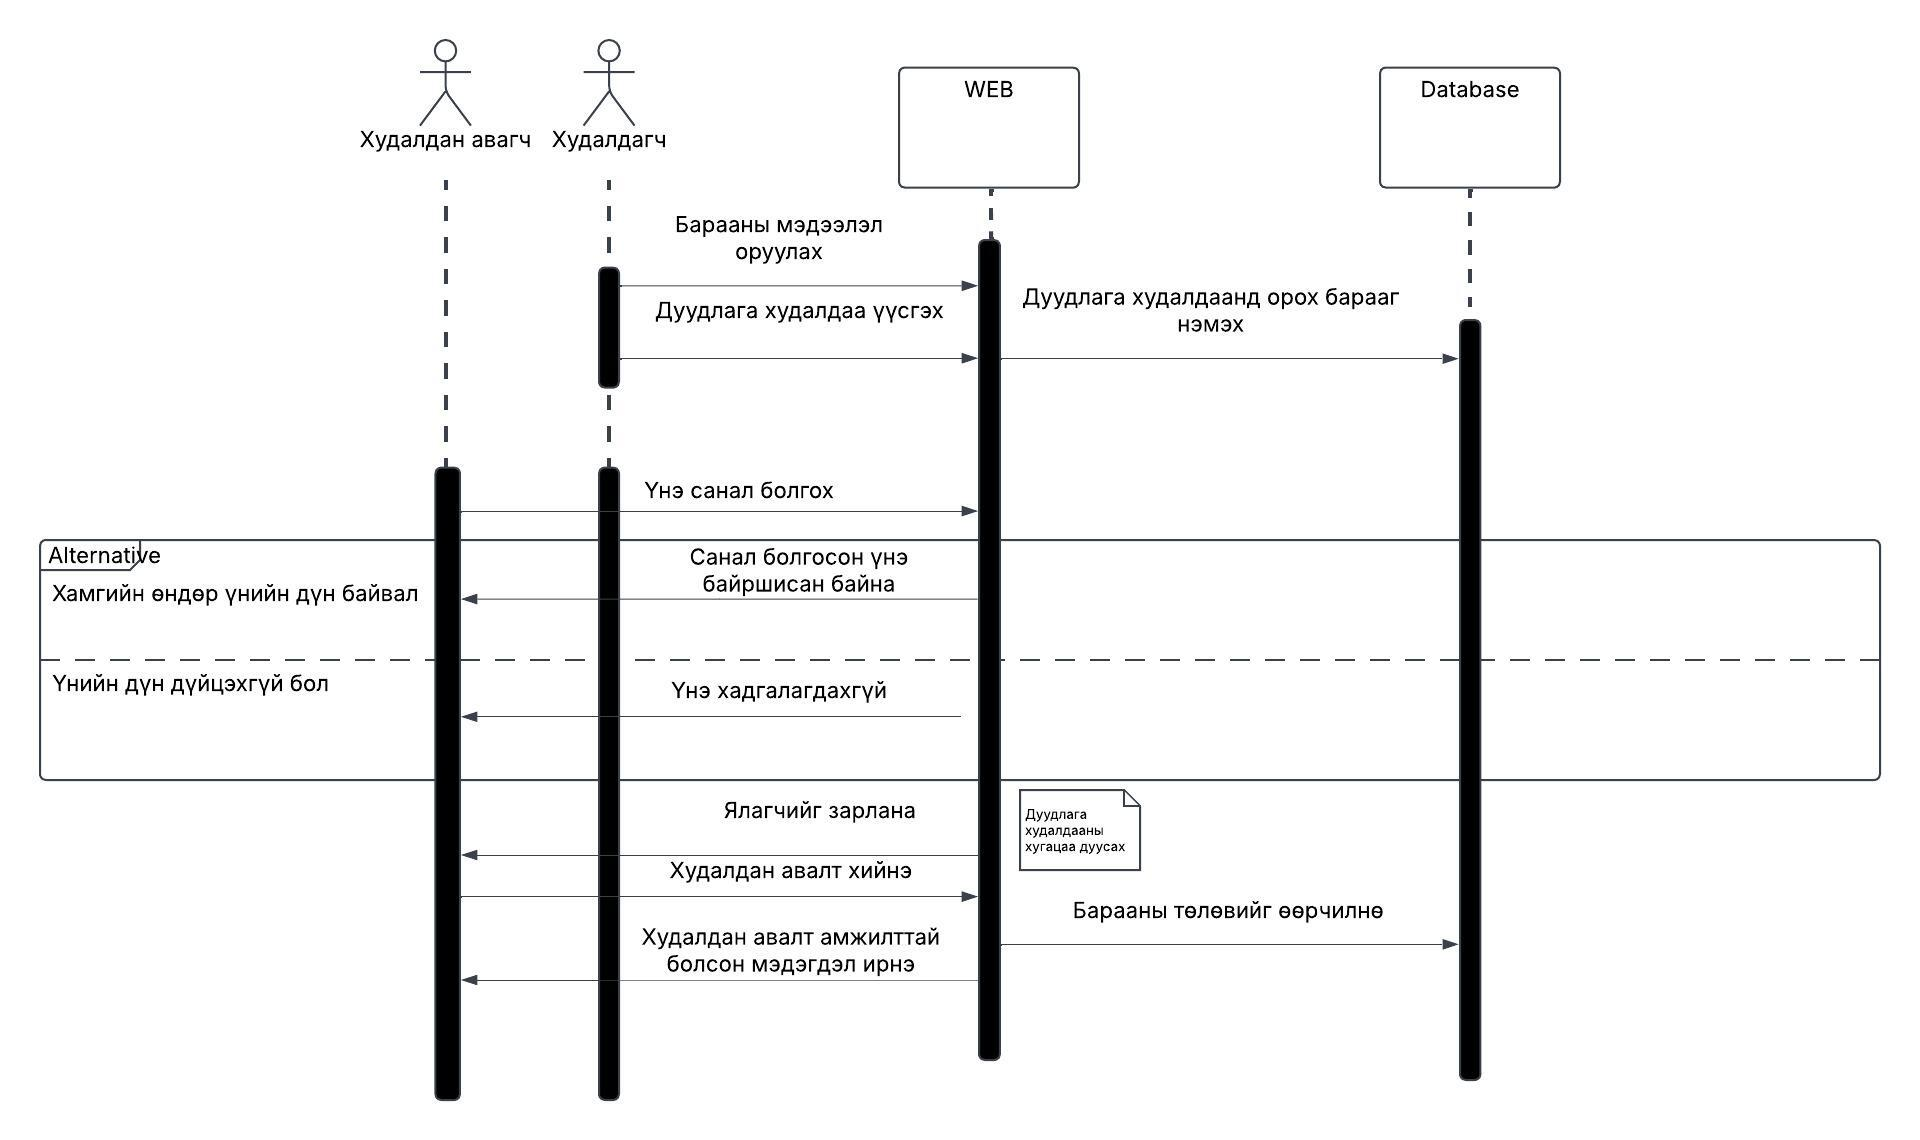
\includegraphics[width=1\textwidth,height=0.8\textheight]{Diagrams/Blank diagram}
    \caption{Үнэ санал болгох дарааллын диаграм}
    \label{fig:shop}
\end{figure}
\clearpage
\section{Төлөвийн диаграм}
\begin{figure}[htbp]
    \centering
    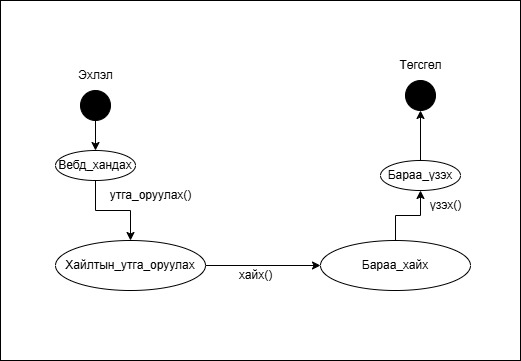
\includegraphics[scale=0.8]{Diagrams/tolow}
    \caption{Хайлт хийх төлөвийн диаграм}
    \label{fig:state1}
\end{figure}

\begin{figure}[htbp]
    \centering
    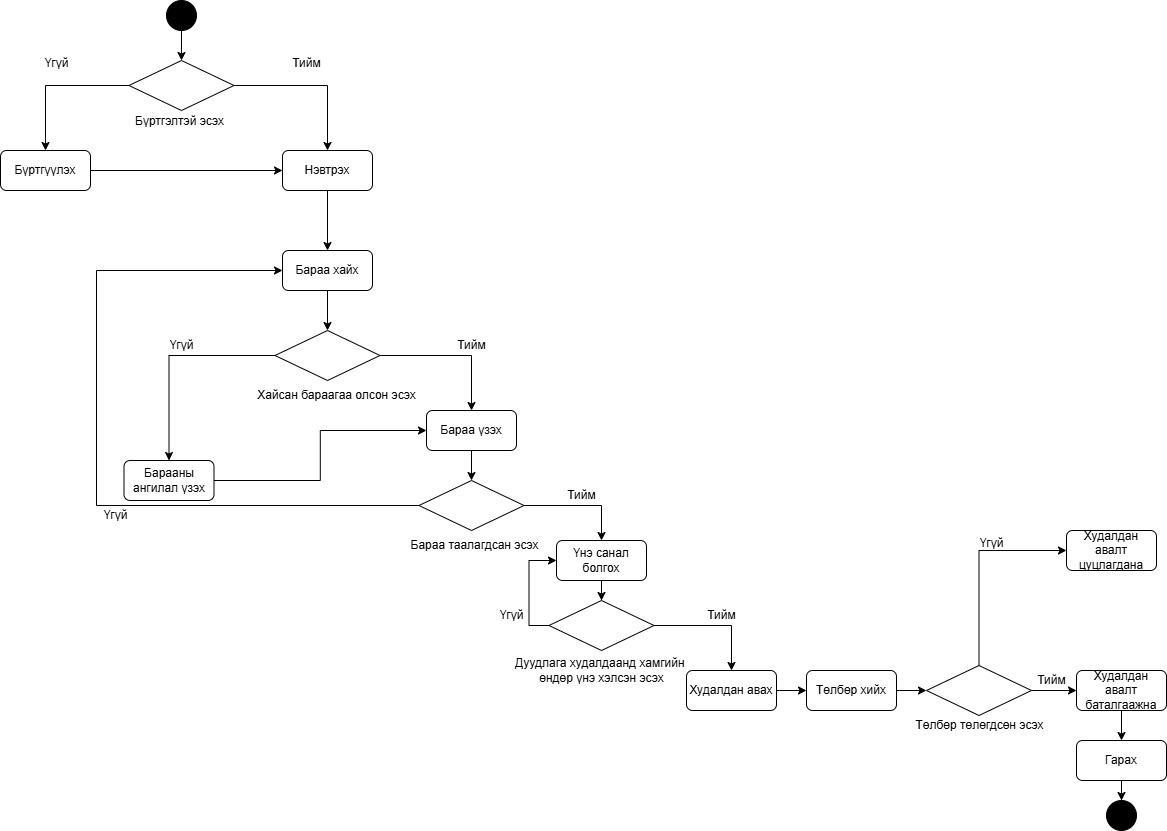
\includegraphics[width=1\textwidth,height=0.7\textheight]{Diagrams/tolow1}
    \caption{Худалдан авалт хийх төлөвийн диаграм}
    
    \label{fig:state2}
\end{figure}

\begin{figure}[htbp]
    \centering
    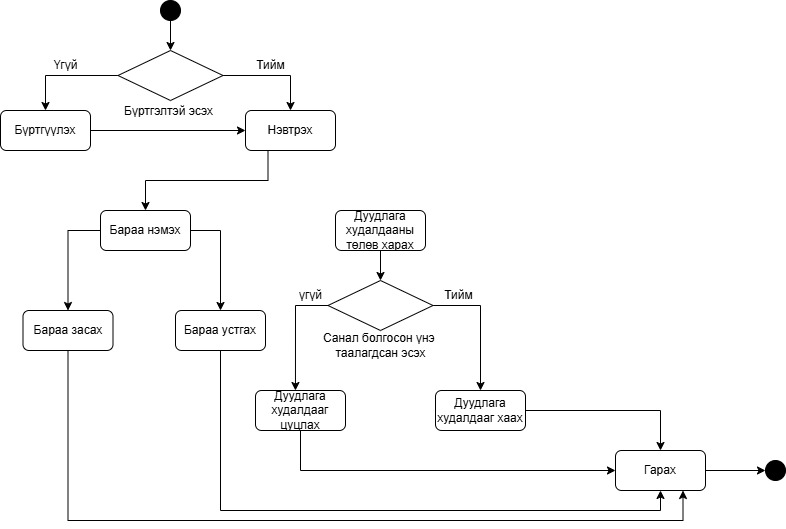
\includegraphics[width=0.9\textwidth,height=0.7\textheight]{Diagrams/tolow2}
    \caption{Бараа нэмэх төлөвийн диаграм}
    \label{fig:state3}
\end{figure}
\clearpage

\section{Үйл ажиллагааны диаграм}
\begin{figure}[htbp]
    \centering
    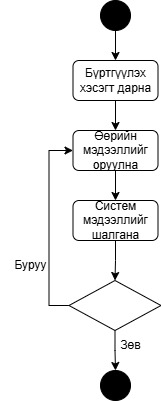
\includegraphics[width=0.3\textwidth]{Diagrams/uilajillagaa}
    \caption{Бүртгүүлэх үйл ажиллагааны диаграм }
    \label{fig:ch2-activity1}
\end{figure}

\clearpage

\begin{figure}[htbp]
    \centering
    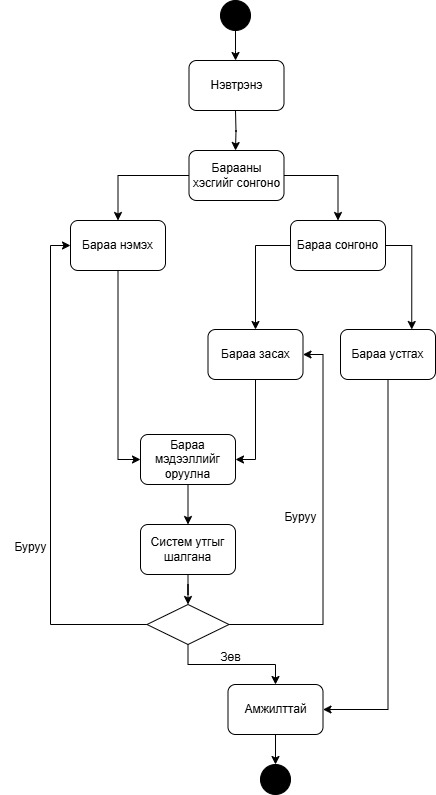
\includegraphics[width=0.7\textwidth]{Diagrams/uilajillagaa2}
    \caption{бараа нэмэх үйл ажиллагааны диаграм}
    \label{fig:activity2}
\end{figure}

%-------------------------------------------------------------------------------

% \section{Бүлгийн дүгнэлт}
% Хэрэглэгчийн шаардлагаа тодорхойлж тодорхойлсон шаардлага бүрээ нягтлан хянаж функционал болон фунционал бусаар нь ялгасан. Функционал шаардлага дээрээ үндэслэн юз кейс диаграмаа гаргасан ба бүх  юзкейс бүрт тодорхойлолт гаргасан. Мөн тодорхойлолт бичсэн юзкейс диаграм бүртээ үйл ажиллагааны диаграм зурсан үйл ажиллагааг нь илүү нарийн ойлгомжтой болгож өгч байна.

